%% abtex2-modelo-trabalho-academico.tex, v-1.9.7 laurocesar
%% Copyright 2012-2018 by abnTeX2 group at http://www.abntex.net.br/ 
%%
%% This work may be distributed and/or modified under the
%% conditions of the LaTeX Project Public License, either version 1.3
%% of this license or (at your option) any later version.
%% The latest version of this license is in
%%   http://www.latex-project.org/lppl.txt
%% and version 1.3 or later is part of all distributions of LaTeX
%% version 2005/12/01 or later.
%%
%% This work has the LPPL maintenance status `maintained'.
%% 
%% The Current Maintainer of this work is the abnTeX2 team, led
%% by Lauro César Araujo. Further information are available on 
%% http://www.abntex.net.br/
%%
%% This work consists of the files abntex2-modelo-trabalho-academico.tex,
%% abntex2-modelo-include-comandos and abntex2-modelo-references.bib
%%

% ------------------------------------------------------------------------
% ------------------------------------------------------------------------
% abnTeX2: Modelo de Trabalho Academico (tese de doutorado, dissertacao de
% mestrado e trabalhos monograficos em geral) em conformidade com 
% ABNT NBR 14724:2011: Informacao e documentacao - Trabalhos academicos -
% Apresentacao
% ------------------------------------------------------------------------
% ------------------------------------------------------------------------

\documentclass[
	% -- opções da classe memoir --
	12pt,				% tamanho da fonte
%	openright,			% capítulos começam em pág ímpar (insere página vazia caso preciso)
%	twoside,			% para impressão em recto e verso. Oposto a oneside
	oneside,
	a4paper,			% tamanho do papel. 
	% -- opções da classe abntex2 --
	%chapter=TITLE,		% títulos de capítulos convertidos em letras maiúsculas
	%section=TITLE,		% títulos de seções convertidos em letras maiúsculas
	%subsection=TITLE,	% títulos de subseções convertidos em letras maiúsculas
	%subsubsection=TITLE,% títulos de subsubseções convertidos em letras maiúsculas
	% -- opções do pacote babel --
	english,			% idioma adicional para hifenização
	spanish,			% idioma adicional para hifenização
	brazil				% o último idioma é o principal do documento
	]{abntex2}

% ---
% Pacotes básicos 
% ---
\usepackage{lmodern}			% Usa a fonte Latin Modern			
\usepackage[T1]{fontenc}		% Selecao de codigos de fonte.
\usepackage[utf8]{inputenc}		% Codificacao do documento (conversão automática dos acentos)
\usepackage{indentfirst}		% Indenta o primeiro parágrafo de cada seção.
\usepackage{color}				% Controle das cores
\usepackage{graphicx}			% Inclusão de gráficos
\usepackage{caption}
%\usepackage{longfigure}
\usepackage{subcaption}
%\usepackage[caption = false]{subfig}
\graphicspath{{images/}{../images/}}
\usepackage{longtable}
\usepackage{microtype} 			% para melhorias de justificação
\usepackage{lscape} % para colocar conteúdo (e.g. Imagens) em modo paisagem
\usepackage{enumitem} % para usar algarismos romanos em listas ordenadas
\usepackage{geometry}
\usepackage{pdfpages}
% ---
		
% ---
% Pacotes adicionais, usados apenas no âmbito do Modelo Canônico do abnteX2
% ---
\usepackage{lipsum}				% para geração de dummy text
% ---

% ---
% Pacotes de citações
% ---
\usepackage[brazilian,hyperpageref]{backref}	 % Paginas com as citações na bibl
\usepackage[alf]{abntex2cite}	% Citações padrão ABNT


%Pacote para usar multiplos arquivos
\usepackage{subfiles} % Importa outros arquivos no arquivo tex principal

% --- 
% CONFIGURAÇÕES DE PACOTES
% --- 
% ---
% Configurações do pacote backref
% Usado sem a opção hyperpageref de backref
\renewcommand{\backrefpagesname}{Citado na(s) página(s):~}
% Texto padrão antes do número das páginas
\renewcommand{\backref}{}
% Define os textos da citação
\renewcommand*{\backrefalt}[4]{
	\ifcase #1 %
		Nenhuma citação no texto.%
	\or
		Citado na página #2.%
	\else
		Citado #1 vezes nas páginas #2.%
	\fi}%
% ---
\hyphenation{Pseu-do-myr-me-ci-nae}
% ---
% Informações de dados para CAPA e FOLHA DE ROSTO
% ---
\titulo{FILOGENÔMICA MITOCONDRIAL SEM CUSTOS: UMA PROVA DE CONCEITO COM FORMIGAS DA SUBFAMÍLIA PSEUDOMYRMECINAE  (HYMENOPTERA : FORMICIDAE)}
\autor{Gabriel Alves Vieira}
\local{Brasil}
\data{Março de 2019}
\orientador{Dr. Francisco Prosdocimi}
%\coorientador{Equipe \abnTeX}
\instituicao{%
  Ministério da Educação
  \par
  Universidade Federal do Rio de Janeiro 
  \par
  Instituto de Bioquímica Médica Leopoldo de Meis
  }
\tipotrabalho{Tese (Doutorado)}
% O preambulo deve conter o tipo do trabalho, o objetivo, 
% o nome da instituição e a área de concentração 
\preambulo{Dissertação apresentada ao Programa de Pós-Graduação em Química Biológica, Instituto de Bioquímica Médica Leopoldo de Meis, Universidade Federal do Rio de Janeiro, como parte dos requisitos para obtenção do título de Mestre em Química Biológica.}
% ---


% ---
% Configurações de aparência do PDF final

% alterando o aspecto da cor azul
\definecolor{blue}{RGB}{41,5,195}

% informações do PDF
\makeatletter
\hypersetup{
     	%pagebackref=true,
		pdftitle={\@title}, 
		pdfauthor={\@author},
    	pdfsubject={\imprimirpreambulo},
	    pdfcreator={LaTeX with abnTeX2},
		pdfkeywords={abnt}{latex}{abntex}{abntex2}{trabalho acadêmico}, 
		colorlinks=true,       		% false: boxed links; true: colored links
    	linkcolor=blue,          	% color of internal links
    	citecolor=blue,        		% color of links to bibliography
    	filecolor=magenta,      		% color of file links
		urlcolor=blue,
		bookmarksdepth=4
}
\makeatother
% --- 

% ---
% Posiciona figuras e tabelas no topo da página quando adicionadas sozinhas
% em um página em branco. Ver https://github.com/abntex/abntex2/issues/170
\makeatletter
\setlength{\@fptop}{5pt} % Set distance from top of page to first float
\makeatother
% ---

% ---
% Possibilita criação de Quadros e Lista de quadros.
% Ver https://github.com/abntex/abntex2/issues/176
%
\newcommand{\quadroname}{Quadro}
\newcommand{\listofquadrosname}{Lista de quadros}

\newfloat[chapter]{quadro}{loq}{\quadroname}
\newlistof{listofquadros}{loq}{\listofquadrosname}
\newlistentry{quadro}{loq}{0}

% configurações para atender às regras da ABNT
\setfloatadjustment{quadro}{\centering}
\counterwithout{quadro}{chapter}
\renewcommand{\cftquadroname}{\quadroname\space} 
\renewcommand*{\cftquadroaftersnum}{\hfill--\hfill}
\renewcommand{\listadesiglasname}{Lista de Abreviaturas e Siglas}

\setfloatlocations{quadro}{hbtp} % Ver https://github.com/abntex/abntex2/issues/176
% ---

% --- 
% Espaçamentos entre linhas e parágrafos 
% --- 

% O tamanho do parágrafo é dado por:
\setlength{\parindent}{1.3cm}

% Controle do espaçamento entre um parágrafo e outro:
\setlength{\parskip}{0.2cm}  % tente também \onelineskip

% ---
% compila o indice
% ---
\makeindex
% ---

% ----
% Início do documento
% ----
\begin{document}

% Seleciona o idioma do documento (conforme pacotes do babel)
%\selectlanguage{english}
\selectlanguage{brazil}

% Retira espaço extra obsoleto entre as frases.
\frenchspacing 

% ----------------------------------------------------------
% ELEMENTOS PRÉ-TEXTUAIS
% ----------------------------------------------------------
% \pretextual

% ---
% Capa
% ---
\imprimircapa
% ---

% ---
% Folha de rosto
% (o * indica que haverá a ficha bibliográfica)
% ---
\imprimirfolhaderosto*
% ---

% ---
% Inserir a ficha bibliografica
% ---

% Isto é um exemplo de Ficha Catalográfica, ou ``Dados internacionais de
% catalogação-na-publicação''. Você pode utilizar este modelo como referência. 
% Porém, provavelmente a biblioteca da sua universidade lhe fornecerá um PDF
% com a ficha catalográfica definitiva após a defesa do trabalho. Quando estiver
% com o documento, salve-o como PDF no diretório do seu projeto e substitua todo
% o conteúdo de implementação deste arquivo pelo comando abaixo:
%
% \begin{fichacatalografica}
%     \includepdf{fig_ficha_catalografica.pdf}
% \end{fichacatalografica}

\begin{fichacatalografica}
	\sffamily
	\vspace*{\fill}					% Posição vertical
	\begin{center}					% Minipage Centralizado
	\fbox{\begin{minipage}[c][8cm]{13.5cm}		% Largura
	\small
	\imprimirautor
	%Sobrenome, Nome do autor
	
	\hspace{0.5cm} \imprimirtitulo  / \imprimirautor. --
	\imprimirlocal, \imprimirdata-
	
	\hspace{0.5cm} \thelastpage p. : il. (algumas color.) ; 30 cm.\\
	
	\hspace{0.5cm} \imprimirorientadorRotulo~\imprimirorientador\\
	
	\hspace{0.5cm}
	\parbox[t]{\textwidth}{\imprimirtipotrabalho~--~\imprimirinstituicao,
	\imprimirdata.}\\
	
	\hspace{0.5cm}
		1. Palavra-chave1.
		2. Palavra-chave2.
		2. Palavra-chave3.
		I. Orientador.
		II. Universidade xxx.
		III. Faculdade de xxx.
		IV. Título 			
	\end{minipage}}
	\end{center}
\end{fichacatalografica}
% ---

% ---
% Inserir errata
% ---
%\begin{errata}
%Elemento opcional da \citeonline[4.2.1.2]{NBR14724:2011}. Exemplo:

%\vspace{\onelineskip}

%FERRIGNO, C. R. A. \textbf{Tratamento de neoplasias ósseas apendiculares com
%reimplantação de enxerto ósseo autólogo autoclavado associado ao plasma
%rico em plaquetas}: estudo crítico na cirurgia de preservação de membro em
%cães. 2011. 128 f. Tese (Livre-Docência) - Faculdade de Medicina Veterinária e
%Zootecnia, Universidade de São Paulo, São Paulo, 2011.

%\begin{table}[htb]
%\center
%\footnotesize
%\begin{tabular}{|p{1.4cm}|p{1cm}|p{3cm}|p{3cm}|}
% \hline
% \textbf{Folha} & \textbf{Linha}  & \textbf{Onde se lê}  & \textbf{Leia-se}  \\
%  \hline
%    1 & 10 & auto-conclavo & autoconclavo\\
%   \hline
%\end{tabular}
%\end{table}

%\end{errata}
% ---

% ---
% Inserir folha de aprovação
% ---

% Isto é um exemplo de Folha de aprovação, elemento obrigatório da NBR
% 14724/2011 (seção 4.2.1.3). Você pode utilizar este modelo até a aprovação
% do trabalho. Após isso, substitua todo o conteúdo deste arquivo por uma
% imagem da página assinada pela banca com o comando abaixo:
%
% \begin{folhadeaprovacao}
% \includepdf{folhadeaprovacao_final.pdf}
% \end{folhadeaprovacao}
%
\begin{folhadeaprovacao}

\begin{center}
      \ABNTEXchapterfont\imprimirtitulo
      \vspace{\fill}
      \ABNTEXchapterfont\large\imprimirautor
      \vspace{\fill}
	\begin{flushleft}
		\ABNTEXchapterfont\large\imprimirpreambulo\vfill
		 
		Aprovado em: 26/03/2019
	\end{flushleft}
	BANCA EXAMINADORA
	\vspace{\fill}
	\hrule\textbf{\imprimirorientador} \\ Prof. Adjunto do Instituto de Bioquímica Médica Leopoldo de Meis da Universidade Federal do Rio de Janeiro – UFRJ
	\vspace{\fill}
	\hrule\textbf{Drª. Carla Ribeiro Polycarpo} \\ Profª. Associada do Instituto de Bioquímica Médica Leopoldo de Meis da Universidade Federal do Rio de Janeiro – UFRJ
	\vspace{\fill}
	\hrule\textbf{Drª Ana Carolina Martins Junqueira} \\ Profª. Adjunta do Instituto de Bioquímica Médica Leopoldo de Meis da Universidade Federal do Rio de Janeiro – UFRJ
	\vspace{\fill}
	\hrule\textbf{Dr. Marcus Fernandes de Oliveira} \\ Prof. Adjunto do Instituto de Bioquímica Médica Leopoldo de Meis da Universidade Federal do Rio de Janeiro – UFRJ
	\vspace{\fill}
	\hrule\textbf{Suplente externo: Dr. Marcelo Weksler} \\ Prof. Titular do Programa de Pós-Graduação em Zoologia do Museu Nacional da Universidade Federal do Rio de Janeiro - UFRJ
	\vspace{\fill}
	\hrule\textbf{Revisor: Dr.  Fernando Lucas Palhano Soares} \\ Prof. Adjunto do Instituto de Bioquímica Médica Leopoldo de Meis da Universidade Federal do Rio de Janeiro – UFRJ \\
\end{center}
  
\end{folhadeaprovacao}
% ---

% ---
% Dedicatória
% ---
%\begin{dedicatoria}
%   \vspace*{\fill}
%   \centering
%   \noindent
%   \textit{ Este trabalho é dedicado às crianças adultas que,\\
%   quando pequenas, sonharam em se tornar cientistas.} \vspace*{\fill}
%\end{dedicatoria}
% ---

% ---
% Agradecimentos
% ---
\begin{agradecimentos}
Aos meus pais que, apesar da enorme vontade de me ter ao lado deles, demonstraram seu amor ao darem apoio incondicional a um filho que, tal qual Brás Cubas, foi dominado por uma idéia fixa: ver e aprender mais sobre bioinformática e o mundo.

À Agatinha, minha mafagafa e companheira de todos os momentos, com a qual constituí família e cresci como pessoa. Abro um sorriso cada vez que encontro uma “AGATA” em alguma mitocôndria e me lembro de como sou sortudo. Completamente desprovido de dons artísticos para te escrever músicas ou poemas, o melhor que consigo fazer é dedicar todas essas sequências, junto com meu coração, a ti.

Aos meus filhos: Seth, que vive roubando meu cobertor e pulando no meu colo sem ser convidado; e Bílquis, que só quer saber de me afofar com suas garrinhas afiadas e me trazer proteína na forma de lagartos (vivos, mortos ou em uma estranha mescla dos dois estados). Amo muito ambos e sem eles não seria plenamente feliz.

Ao Exmo. Prof. Dr. Francisco Prosdocimi, por ter lido um email (redigido com pressa e provavelmente contendo múltiplos erros ortográficos) no final de 2016 de um cara meio maluco e afobado que queria estudar bioinformática. Mais do que isso, agradeço por ele ter depositado confiança no dito cujo e aceitado orientá-lo.

A todos os meus colegas do LAMPADA/Laboratório de Genômica e Biodiversidade, em especial à Ana e Deise. Sem a ajuda e apoio de vocês, meu trabalho seria muito menos divertido /empolgante e eu certamente teria traçado arestas menos satisfatórias na tentativa de resolver esse grafo de dois anos que foi meu mestrado.

A todos aqueles que geraram e disponibilizaram os \textit{datasets} utilizados aqui. Se eu não tivesse tido o privilégio de subir nos ombros desses gigantes, esse trabalho não existiria. Embora nós tenhamos explorado perguntas, metodologias e evidências diferentes ao nos aventurar por esses dados, acredito que comungamos de um objetivo comum: promover o avanço de uma ciência tão aberta e colaborativa quanto possível.

À CAPES e demais agências de fomento, por darem suporte a esse trabalho

\end{agradecimentos}
% ---

% ---
% Epígrafe
% ---
\begin{epigrafe}
    \vspace*{\fill}
	\begin{flushright}
		\textit{
		``I like the hand we’ve been dealt.'' \\
		(Uncharted 4: A Thief’s End - 2016)
	}
	\end{flushright}
\end{epigrafe}
% ---

% ---
% RESUMOS
% ---

% resumo em português
\setlength{\absparsep}{18pt} % ajusta o espaçamento dos parágrafos do resumo
\begin{resumo}
 O advento do Sequenciamento de Nova Geração reduziu os custos de sequenciamento e aumentou o número de projetos genômicos para uma enorme gama de organismos, gerando uma quantidade sem precedentes de conjuntos de dados genômicos publicamente disponíveis. Muitas vezes, apenas uma pequena fração da relevância dos dados produzidos pelos pesquisadores é contemplada em seus trabalhos. Este fato permite que os dados gerados sejam reciclados em outros projetos ao redor do mundo. A montagem de mitogenomas completos é frequentemente negligenciada, embora seja útil para entender as relações evolutivas entre táxons, especialmente aqueles que apresentam baixa amostragem de mtDNA ao nível de gêneros e famílias. Esse é exatamente o caso das formigas (Hymenoptera: Formicidae) e, mais especificamente, da subfamília Pseudomyrmecinae, um grupo de formigas arbóreas com vários casos de coevolução convergente mas sem qualquer sequência mitocondrial completa disponível. Nesta dissertação reunimos, anotamos e realizamos análises genômicas comparativas de 14 novos genomas mitocondriais completos de espécies de Pseudomyrmecinae,  usando apenas os conjuntos de dados públicos disponíveis no Sequence Read Archive (SRA). Utilizamos todos os mitogenomas completos disponíveis para formigas para estudar a conservação da ordem gênica e também para gerar duas árvores filogenéticas usando (i) conjunto concatenado de 13 genes mitocondriais e (ii) as seqüências mitocondriais completas. Embora as topologias das árvores tenham divergido sutilmente umas das outras (e de estudos anteriores), nossos resultados confirmam várias relações conhecidas e geram novas evidências para a classificação de grupos irmão dentro de Pseudomyrmecinae. Também realizamos uma análise de sintenia para a família Formicidae e identificamos possíveis sítios nos quais inserções nucleotídicas ocorreram em mitogenomas de formigas do gênero Pseudomyrmex. Usando uma abordagem de mineração de dados/bioinformática, a dissertação atual aumentou o número de genomas mitocondriais completos disponíveis para formigas de 15 para 29, demonstrando o potencial único dos bancos de dados públicos para estudos mitogenômicos. As amplas aplicações de mitogenomas na pesquisa e a presença de dados mitocondriais em diferentes tipos de dados públicos tornam a abordagem da “mitogenômica no-budget” ideal para estudos moleculares abrangentes, especialmente para taxóns subamostrados.

 \textbf{Palavras-chave}: Pseudomyrmecinae, Mitogenômica, Mineração de dados, Bioinformática, Filogenômica, Biologia evolutiva de formigas, Sequenciamento de nova geração, Dados públicos.
\end{resumo}

% resumo em inglês
\begin{resumo}[Abstract]
 \begin{otherlanguage*}{english}
   The advent of Next Generation Sequencing has reduced sequencing costs and increased genomic projects from a huge amount of organismal taxa, generating an unprecedented amount of genomic datasets publicly available. Often, only a tiny fraction of outstanding relevance of the genome data produced by researchers is used in their works. This fact allows the data generated to be recycled in further projects worldwide. The assembly of complete mitogenomes is frequently overlooked though it is useful to understand evolutionary relationships among taxa, especially those presenting poor mtDNA sampling at the level of genera and families. This is exactly the case for ants (Hymenoptera:Formicidae) and more specifically for the subfamily Pseudomyrmecinae, a group of arboreal ants with several cases of convergent coevolution without any complete mitochondrial sequence available. In this dissertation, we assembled, annotated and performed comparative genomics analyses of 14 new complete mitochondrial genomes from Pseudomyrmecinae species relying solely on public datasets available from the Sequence Read Archive (SRA). We used all complete mitogenomes available for ants to study the gene order conservation and also to generate two phylogenetic trees using both (i) concatenated set of 13 mitochondrial genes and (ii) the whole mitochondrial sequences. Even though the tree topologies diverged subtly from each other (and from previous studies), our results confirm several known relationships and generate new evidences for sister clade classification inside Pseudomyrmecinae clade. We also performed a synteny analysis for Formcidae and identified possible sites in which nucleotidic insertions happened in mitogenomes of pseudomyrmecine ants. Using a data mining/bioinformatics approach, the current dissertation increased the number of complete mitochondrial genomes available for ants from 15 to 29, demonstrating the unique potential of public databases for mitogenomics studies. The wide applications of mitogenomes in research and presence of mitochondrial data in different public dataset types makes the “no budget mitogenomics” approach ideal for comprehensive molecular studies, especially for subsampled taxa.

   \vspace{\onelineskip}
 
   \noindent 
   \textbf{Keywords}: Pseudomyrmecinae, Mitogenomics, Data mining, Bioinformatics, Phylogenomics, Ant evolutionary biology, Next Generation Sequencing, Public data. 
 \end{otherlanguage*}
\end{resumo}

% resumo em francês 
%\begin{resumo}[Résumé]
% \begin{otherlanguage*}{french}
%    Il s'agit d'un résumé en français.
% 
%   \textbf{Mots-clés}: latex. abntex. publication de textes.
% \end{otherlanguage*}
%\end{resumo}

% resumo em espanhol
%\begin{resumo}[Resumen]
% \begin{otherlanguage*}{spanish}
%   Este es el resumen en español.
  
%   \textbf{Palabras clave}: latex. abntex. publicación de textos.
% \end{otherlanguage*}
%\end{resumo}
% ---

% ---
% inserir lista de ilustrações
% ---
\pdfbookmark[0]{\listfigurename}{lof}
\listoffigures*
\cleardoublepage
% ---

% ---
% inserir lista de quadros
% ---
%\pdfbookmark[0]{\listofquadrosname}{loq}
%\listofquadros*
%\cleardoublepage
% ---

% ---
% inserir lista de tabelas
% ---
\pdfbookmark[0]{\listtablename}{lot}
\listoftables*
\cleardoublepage
% ---

% ---
% inserir lista de abreviaturas e siglas
% ---
\begin{siglas}
  \item[\textbf{3’OH:}] Hidroxila presente no carbono 3’ de um nucleotídeo
  \item[\textbf{A:}] Amina (base púrica)
  \item[\textbf{ATP6:}] ATP sintase F0 subunidade 6
  \item[\textbf{ATP8:}] ATP sintase F0 subunidade 8
  \item[\textbf{BLAST:}] Basic Local Alignment Search Tool
  \item[\textbf{BLASTp:}] Protein-protein BLAST
  \item[\textbf{BRIG:}] Blast Ring Image Generator
  \item[\textbf{BS:}] Suporte de Bootstrap
  \item[\textbf{C:}] Citosina (base pirimídica)
  \item[\textbf{COX1:}] Citocromo oxidase 1
  \item[\textbf{COX2:}] Citocromo oxidase 2
  \item[\textbf{DDBJ:}] DNA Data Bank of Japan
  \item[\textbf{DNA:}] Ácido desoxirribonucleico
  \item[\textbf{EBI:}] European Bioinformatics Institute
  \item[\textbf{EMBL:}] European Molecular Biology Laboratory
  \item[\textbf{G:}] Guanina (base púrica)
  \item[\textbf{Gpb:}] Giga pares de base (1000000000 bp)
  \item[\textbf{GTR+G+I:}] Modelo de substituição nucleotídica “General Time Reversible + Gamma distributed + Invariant sites”
  \item[\textbf{INSDC:}] International Nucleotide Sequence Database Collaboration
  \item[\textbf{kpb:}] Kilo pares de base (1000 pb)
  \item[\textbf{ML:}] Máxima Verossimilhança
  \item[\textbf{MMG:}] Metagenômica mitocondrial
  \item[\textbf{Mpb:}] Mega pares de base (1000000 pb)
  \item[\textbf{mRNA:}] RNA mensageiro
  \item[\textbf{mtDNA:}] DNA mitocondrial
  \item[\textbf{MYA:}] Milhões de anos atrás
  \item[\textbf{N:}] Base desconhecida
  \item[\textbf{NCBI:}] National Center for Biotechnology Information 
  \item[\textbf{NGS:}] Sequenciamento de Nova Geração
  \item[\textbf{ORF:}] Fase aberta de leitura
  \item[\textbf{pb:}] Pares de base
  \item[\textbf{PCG:}] Gene codificador de proteína
  \item[\textbf{PCR:}] Reação em cadeia da polimerase
  \item[\textbf{RNA:}] Ácido ribonucleico
  \item[\textbf{RNA-Seq:}] Sequenciamento de mRNA
  \item[\textbf{rRNA:}] RNA ribossomal
  \item[\textbf{rrnS:}] RNA ribossomal 16S
  \item[\textbf{SBS:}] Sequenciamento por síntese
  \item[\textbf{SRA:}] Sequence Read Archive
  \item[\textbf{T:}] Timina (base pirimídica)
  \item[\textbf{TPA:}] Banco de anotação terceirizada do Genbank
  \item[\textbf{tRNA:}] RNA transportador
  \item[\textbf{trn-X:}] RNA transportador relativo ao aminoácido X
  \item[\textbf{UCE:}] Elementos ultra-conservados
  \item[\textbf{WGS:}] Sequenciamento de genoma completo
\end{siglas}

% ---

% ---
% inserir lista de símbolos
% ---
%\begin{simbolos}
%  \item[$ \Gamma $] Letra grega Gama
%  \item[$ \Lambda $] Lambda
%  \item[$ \zeta $] Letra grega minúscula zeta
%  \item[$ \in $] Pertence
%\end{simbolos}
% ---

% ---
% inserir o sumario
% ---
\pdfbookmark[0]{\contentsname}{toc}
\tableofcontents*
\cleardoublepage
% ---



% ----------------------------------------------------------
% ELEMENTOS TEXTUAIS
% ----------------------------------------------------------
\textual

% ----------------------------------------------------------
% Introdução (exemplo de capítulo sem numeração, mas presente no Sumário)
% ----------------------------------------------------------
\chapter{Introdução}

\subfile{DISSERTACAO_CAPITULOS/01_INTRODUCAO}

% ----------------------------------------------------------

\chapter{Objetivos}

\section{Objetivos gerais}

\subfile{DISSERTACAO_CAPITULOS/02_OBJETIVOS}

\chapter{Metodologia}

\subfile{DISSERTACAO_CAPITULOS/03_METODOS}

\chapter{Resultados}

\subfile{DISSERTACAO_CAPITULOS/04_RESULTADOS}

\chapter{Discussão}

\subfile{DISSERTACAO_CAPITULOS/05_DISCUSSAO}

\chapter{Perspectivas}

\subfile{DISSERTACAO_CAPITULOS/06_PERSPECTIVAS}

\chapter{Conclusão}

\subfile{DISSERTACAO_CAPITULOS/07_CONCLUSAO}

% ---
% ----------------------------------------------------------
% ELEMENTOS PÓS-TEXTUAIS
% ----------------------------------------------------------
\postextual
% ----------------------------------------------------------

% ----------------------------------------------------------
% Referências bibliográficas
% ----------------------------------------------------------
\bibliography{library}\label{references}

% ----------------------------------------------------------
% Glossário
% ----------------------------------------------------------
%
% Consulte o manual da classe abntex2 para orientações sobre o glossário.
%
%\glossary

% ----------------------------------------------------------
% Apêndices
% ----------------------------------------------------------

% ---
% Inicia os apêndices
% ---
\begin{apendicesenv}

% Imprime uma página indicando o início dos apêndices
\partapendices

% ----------------------------------------------------------
\chapter{Figuras e tabelas adicionais}
% ----------------------------------------------------------

\subfile{DISSERTACAO_CAPITULOS/08_APENDICESA}

% ----------------------------------------------------------
%\chapter{Artigo publicado}
% ----------------------------------------------------------

\chapter{Artigo Publicado}

\includepdf[pages={2-}]{DISSERTACAO_CAPITULOS/08_APENDICESB.pdf}

\end{apendicesenv}
% ---


% ----------------------------------------------------------
% Anexos
% ----------------------------------------------------------

% ---
% Inicia os anexos
% ---
%\begin{anexosenv}

% Imprime uma página indicando o início dos anexos
%\partanexos

% ---
%\chapter{Morbi ultrices rutrum lorem.}
% ---
%\lipsum[30]

% ---
%\chapter{Cras non urna sed feugiat cum sociis natoque penatibus et magnis dis
%parturient montes nascetur ridiculus mus}
% ---

%\lipsum[31]

% ---
%\chapter{Fusce facilisis lacinia dui}
% ---

%\lipsum[32]

%\end{anexosenv}

%---------------------------------------------------------------------
% INDICE REMISSIVO
%---------------------------------------------------------------------
\phantompart
\printindex
%---------------------------------------------------------------------

\end{document}
